\section{Einleitung}
\label{sec:introduction}

SQLino ist bisher auf die Erstellung von Seiten mit Texten und Tabellen
begrenzt. Praktisch relevante Webseiten verwenden allerdings fast ausnahmslos
auch grafische Gestaltungselemente. Darunter fallen zum Beispiel Fotos von im
Text beschriebenen Sachverhalten, bei denen auf Autos gefallene, entwurzelte
Bäumes, Gebirgspanoramen, Strände oder Demonstrationszüge zu sehen sind. Gemäß
dem Motto \enquote{ein Bild sagt mehr als 1000 Worte} profitiert hier der Leser
von den Bildern, solange es sich nicht um unpassende Symbolbilder wie bei
Berichten über Vorfälle im Bereich IT Sicherheit üblich handelt. Darüber hinaus
gibt es auch Sachverhalte die sich kurz und prägnant durch Diagramme, nicht aber
durch Texte erfassen lassen. Dementsprechend ist die Ergänzung um grafische
Inhalte für SQLino sowohl praktisch relevant als auch (vermutlich) für die
Schülerinnen und Schüler \footnote{Zugunsten der leichteren Lesbarkeit wird in
  dieser Thesis auf die Ausdifferenzierung des Geschlechts von Personen im
  Folgenden verzichtet, da es für den Sachverhalt irrelevant ist und den
  Lesefluss stört.  Wenn in dieser Thesis Personen genannt werden, steht   das
  grammatikalische Geschlecht in keinem Zusammenhang zum tatsächliche Geschlecht
  der jeweilig genannten Personen und es sind immer alle Personen gemeint, auf
  die die restliche Beeschreibung zutrifft, unabhängig des Geschlechts.}
motivierend.

\begin{figure}[ht]
  \begin{subfigure}[b]{\columnwidth}
    \includegraphics[width=\columnwidth]{images/introduction-example-before.png}
    \caption{Projektseite mit Tabelle ohne Bilder, Urheber: Marcus Riemer,
      Lizenz: CC-BY}
    \label{fig:comparison-before}
  \end{subfigure}
  \begin{subfigure}[b]{\columnwidth}
    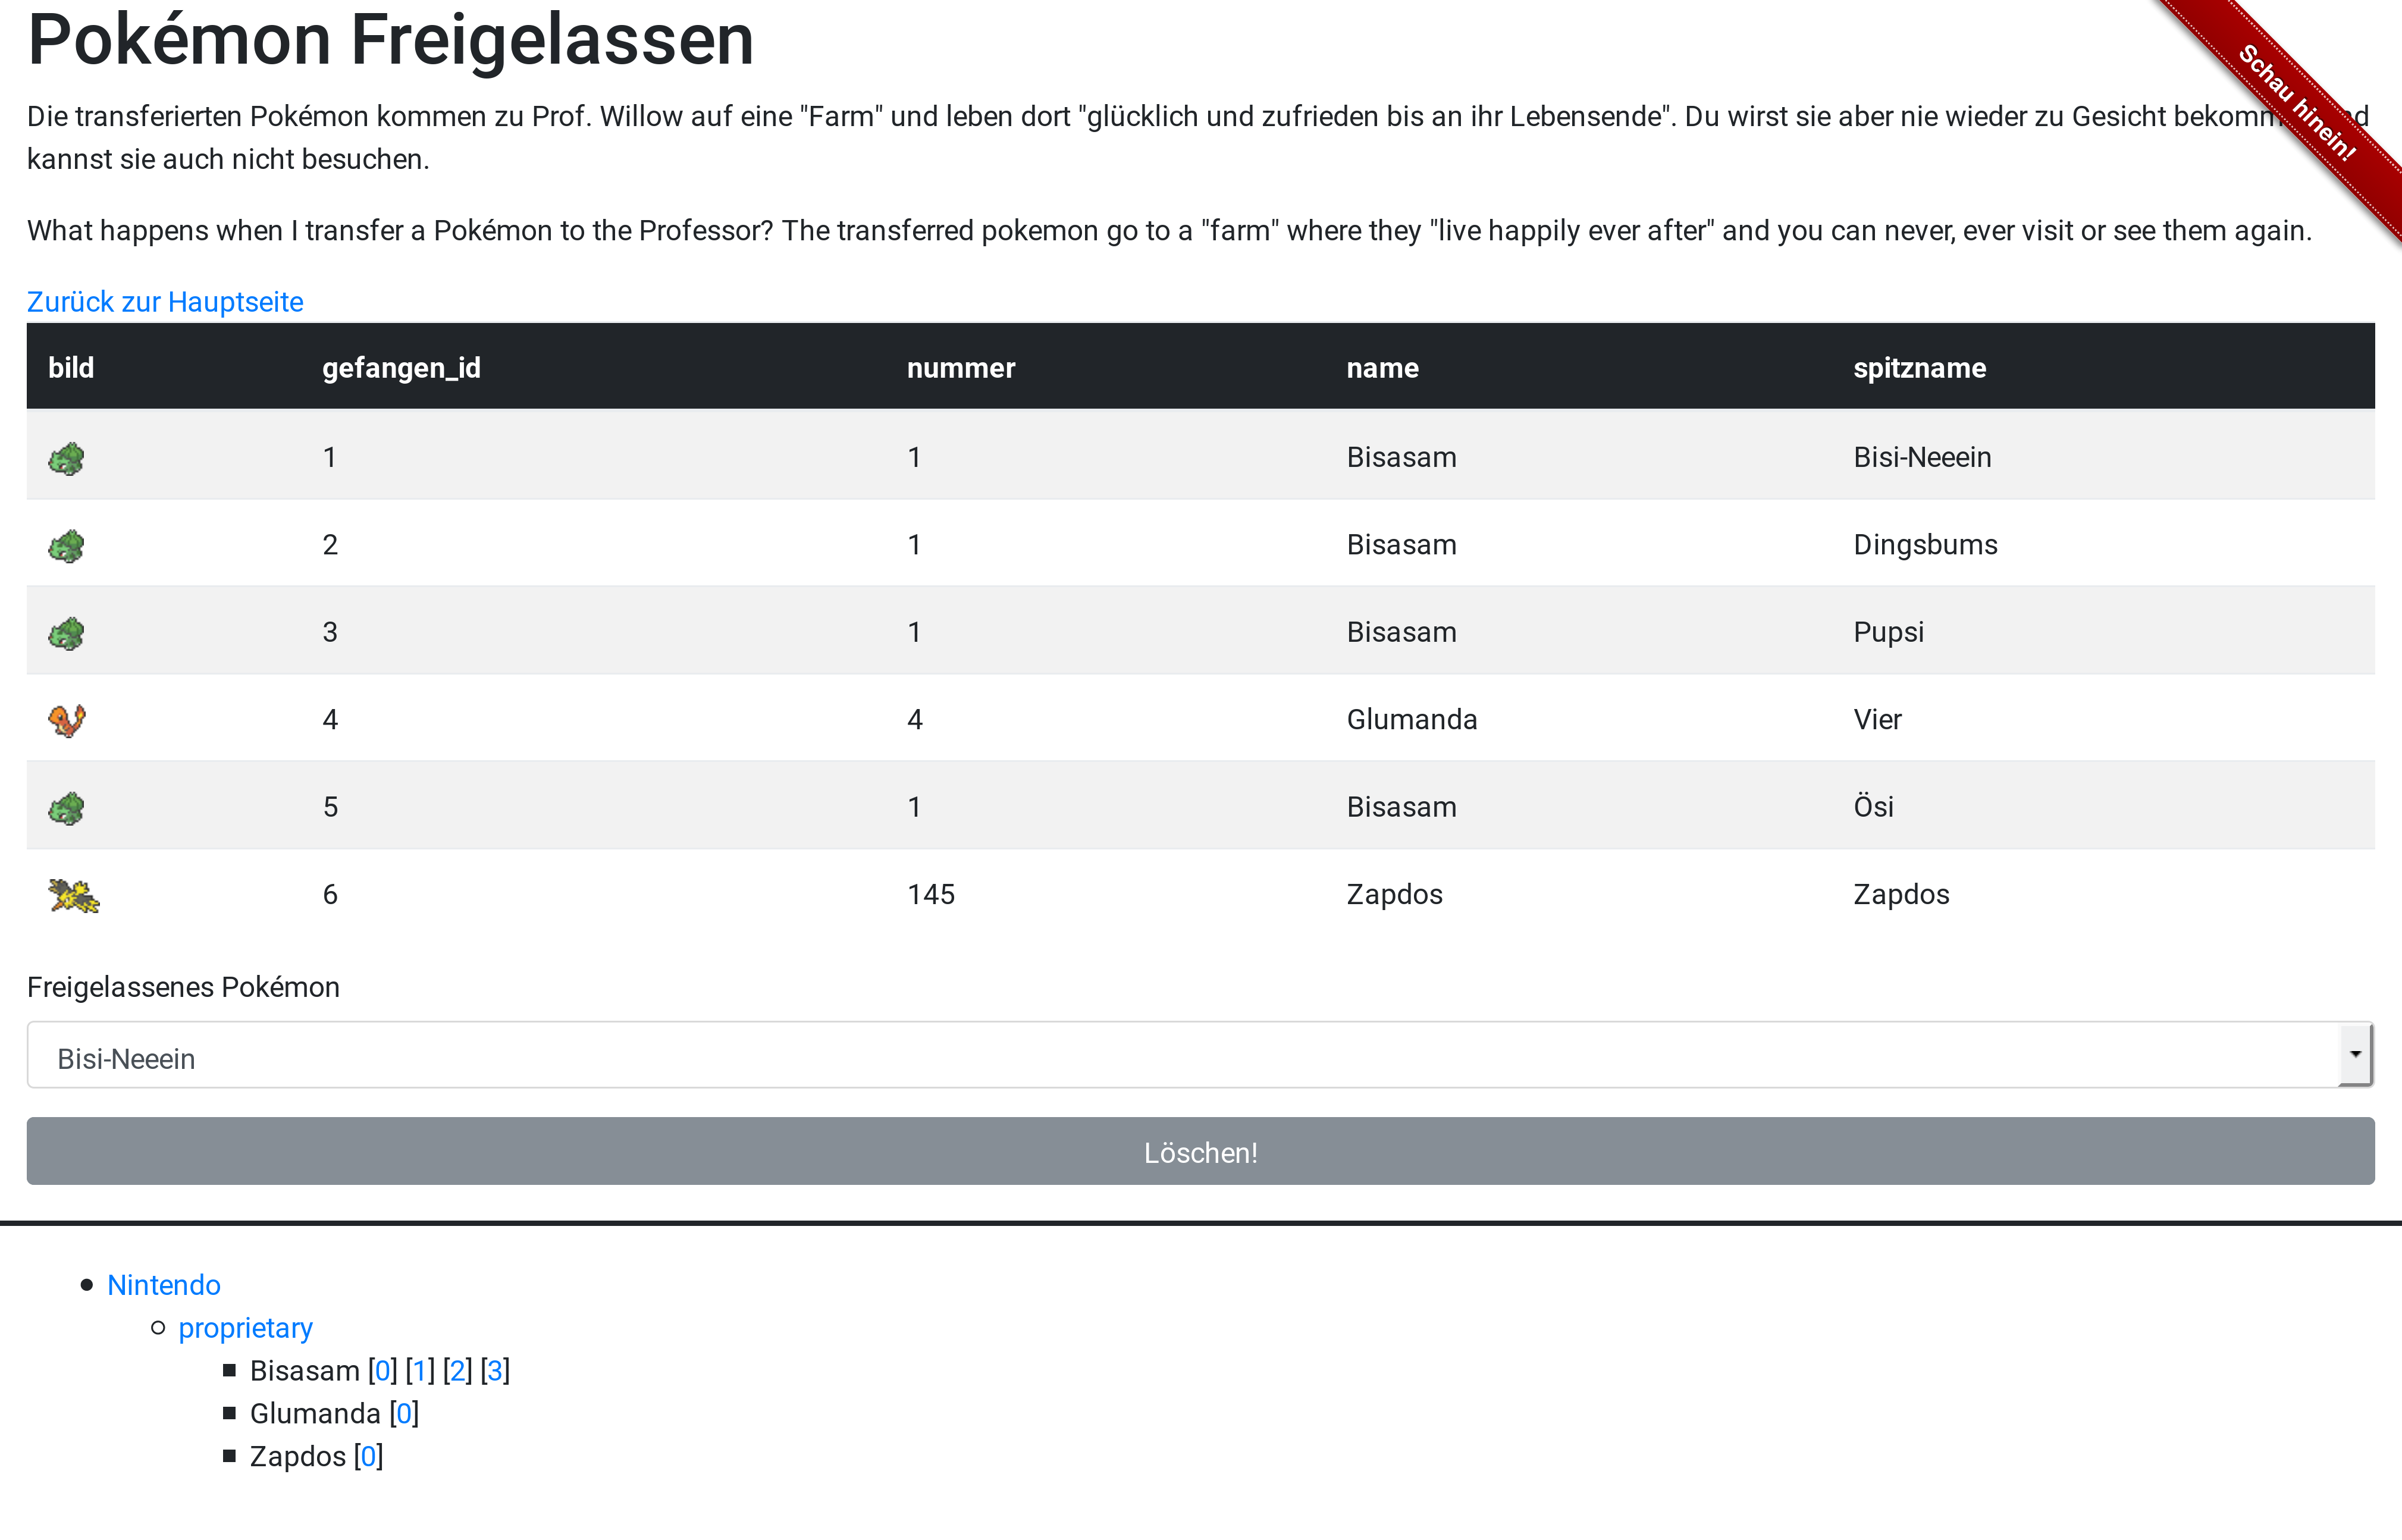
\includegraphics[width=\columnwidth]{images/introduction-example-after.png}
    \caption{Projektseite mit Tabelle mit Bildern aus der Bildverwaltung}
    \label{fig:comparison-after}
  \end{subfigure}
  \caption{Vorher-Nacher Vergleich}
  \label{fig:comparison-before-after}
\end{figure}

Die Verwendung von Bildern auf Webseiten bereitet jedoch auch immer wieder
Probleme. Da sind zum einen technische Günde wie deutlich zu hohen Dateigrößen,
welche Ladezeiten in die Länge ziehen und bei Mobilgeräten das in Deutschland im
Vergleich zu anderen Ländern um Größenordnungen geringere Datenvolumen unötig
schnell aufbrauchen - von der Unbenutzbarkeit solcher Webseiten in den magelhaft
Ausgebauten Mobilfunknetzten im ländlichen Raum und Breitbandanschlüsse, die
ihrem Namen nicht gerecht werden mal ganz abgesehen.

Zum anderen sorgen rechtliche Gründe immer wieder Probleme, die auf die
mangelnde Auseinandersetzung mit dem Urheberrecht und Nutzungslizenzen.
Sogenannte Soziale Netzwerke und Diskussionsplatformen verleiten den Nutzer
Bilder einzustellen und dem Anbieter der Platform laut AGB diverse Rechte an
diesen Bildern zu übertragen. Da der durchschnittliche Nutzer weder die AGB
gelesen hat, noch sich dessen bewusst ist, dass die Befugnis die Rechte an den
Bildern Dritter an den Platformbetreiber weiterzugeben bei besagten Dritten
liegt und nicht bei der eigenen Person.

Beim Umgang mit Bildern soll SQLino die Nutzer für die rechtlichen Aspekte des
Umgangs mit Bildern anderer sensibilisieren und eine technische Lösung bieten,
damit Bilder die Übertragungswege 

Ein weiteres Problem ist die Verwaltung dieser Bilder. Ein Bild wird bei
irgendeinem gerade angesagtem Imagehoster abgelegt, eingebunden und vergessen.
Andere Bilder werden anderswo abgelegt, eingebunden und vergessen. Einige der
Imagehoster liefern nach tausend Aufrufen im Monat das Bild nicht mehr aus ohne
sich dafür bezahlen zu lassen, andere ändern nach einiger Zeit ihr Konzept und
lassen einbetten ihrer Bilder auf fremden Seiten nicht mehr zu und zeigen die
Bilder nur noch auf ihrer eigenen Werbefinanzierten Webseite an und wiederum
andere haben in der zwischenzeit Insolvenz angemeldet und alle dort
gespeicherten Bilder sind nicht mehr verfügbar. Deshalb ist die einzig sinnvoll
anwendbare Methode \todo{bessere formulierung finden} für SQLino die Bilder
selbst zu verwalten.

Diese Thesis beschreibt den Prototypen einer Bildverwaltung für SQLino, die auf
diese Probleme eingeht, indem verwendete Bilder an einem Ort gesammelt und
verwaltet werden, den Bildern Metadaten wie Urheber und Lizenz zugeordnet
werden und dem Betrachter der Webseite dargestellt werden und Bilder beim
ausliefern auf die für das Endgerät geeignete Größe herunterskaliert werden.

Ein weiteres bearbeites Problem ist das Verwalten von Programmabhängigkeiten,
die beim Entwickeln und Testen der Software sowie deren Produktivbetrieb zu
berücksichtigen sind. Das Aufsetzen des Entwicklungssystems, Testsystems und
Produktivsystems ist in der Regel Zeitaufwändig und je nach Betriebssystem und
Zeitpunkt des Einrichtens sehr frustrierend, wenn beispielsweise die aktuelle
Versionskombination in der Packetverwaltung für den Zeitraum einer Woche
fehlerhaft konfiguriert ist und dadurch nur ein Programm, was aber im Projekt
verwendet wird ein bisher nie dagewesenes Fehlverhalten aufweist, allerdings in
genau dieser Woche ein neuer Entwickler versucht das Projekt in Betrieb zu
nehmen. Gleiches gilt für auf externe Infrastruktur ausgelagerte, gemeinhin auch
als cloudbasiert bekannte, Testsysteme, deren zufallsbedinge Fehlkonfiguration
durch ungünstigen Installationszeitpunkt zu unnötigem Mehraufwand in Form von
Fehlersuche unbedingt vermieden werden sollte.

%%% Local Variables:
%%% mode: latex
%%% TeX-master: "thesis"
%%% End:
